\documentclass[titlepage]{article}
\usepackage[margin=.75in]{geometry}
\usepackage{booktabs}
\usepackage{tabularx}
\usepackage{pdfpages}
\usepackage{hyperref}

\setlength{\parindent}{0pt}

\title{CS 451 Group 5:\\Final Summary Document}
\author{Eric Hegnes, Daniel Gildenbrand, Derek Mallon, David Nartey}
\date{March 11, 2019}

\begin{document}
\maketitle
\tableofcontents

\section{Usage}
Building is handled via \href{https://www.docker.com/}{Docker} to provide a unified environment for building
without individual package management.

\subsection{Dependencies}
\begin{itemize}
  \item Docker (\url{https://www.docker.com/get-started})
  \item Docker Compose (\url{https://docs.docker.com/compose/install/})
  \item GNU Make (\url{https://www.gnu.org/software/make/})
\end{itemize}

\subsection{Make Targets}
\begin{tabularx}{\textwidth}{|l|X|}
  \hline
  Target & Description  \\ \hline
  \texttt{all} & Format and run code  \\
  \texttt{fmt} & Format code according to official guidelines  \\
  \texttt{watch} & Watch source files and run tests on change  \\
  \texttt{lint} & Report linting warnings  \\
  \texttt{req-docs} & Generate requirements documentation  \\
  \texttt{test-docs} & Generate test case documentation  \\
  \texttt{final-docs} & Generate final documentation  \\
  \texttt{src-docs} & Generate and serve source documentation  \\
  \texttt{todos} & List stray TODO comments in the source  \\
  \texttt{cov} & Generate coverage report (with branches)*  \\
  \texttt{clean} & Remove generated files \\
  \hline
\end{tabularx}
* \textit{Coverage reporting currently requires a} \texttt{rust} \textit{nightly build
and other dependencies such as} \texttt{lcov}.

\subsection{Building}
Once the dependencies are installed, the game may be run inside a terminal with \texttt{make run}.

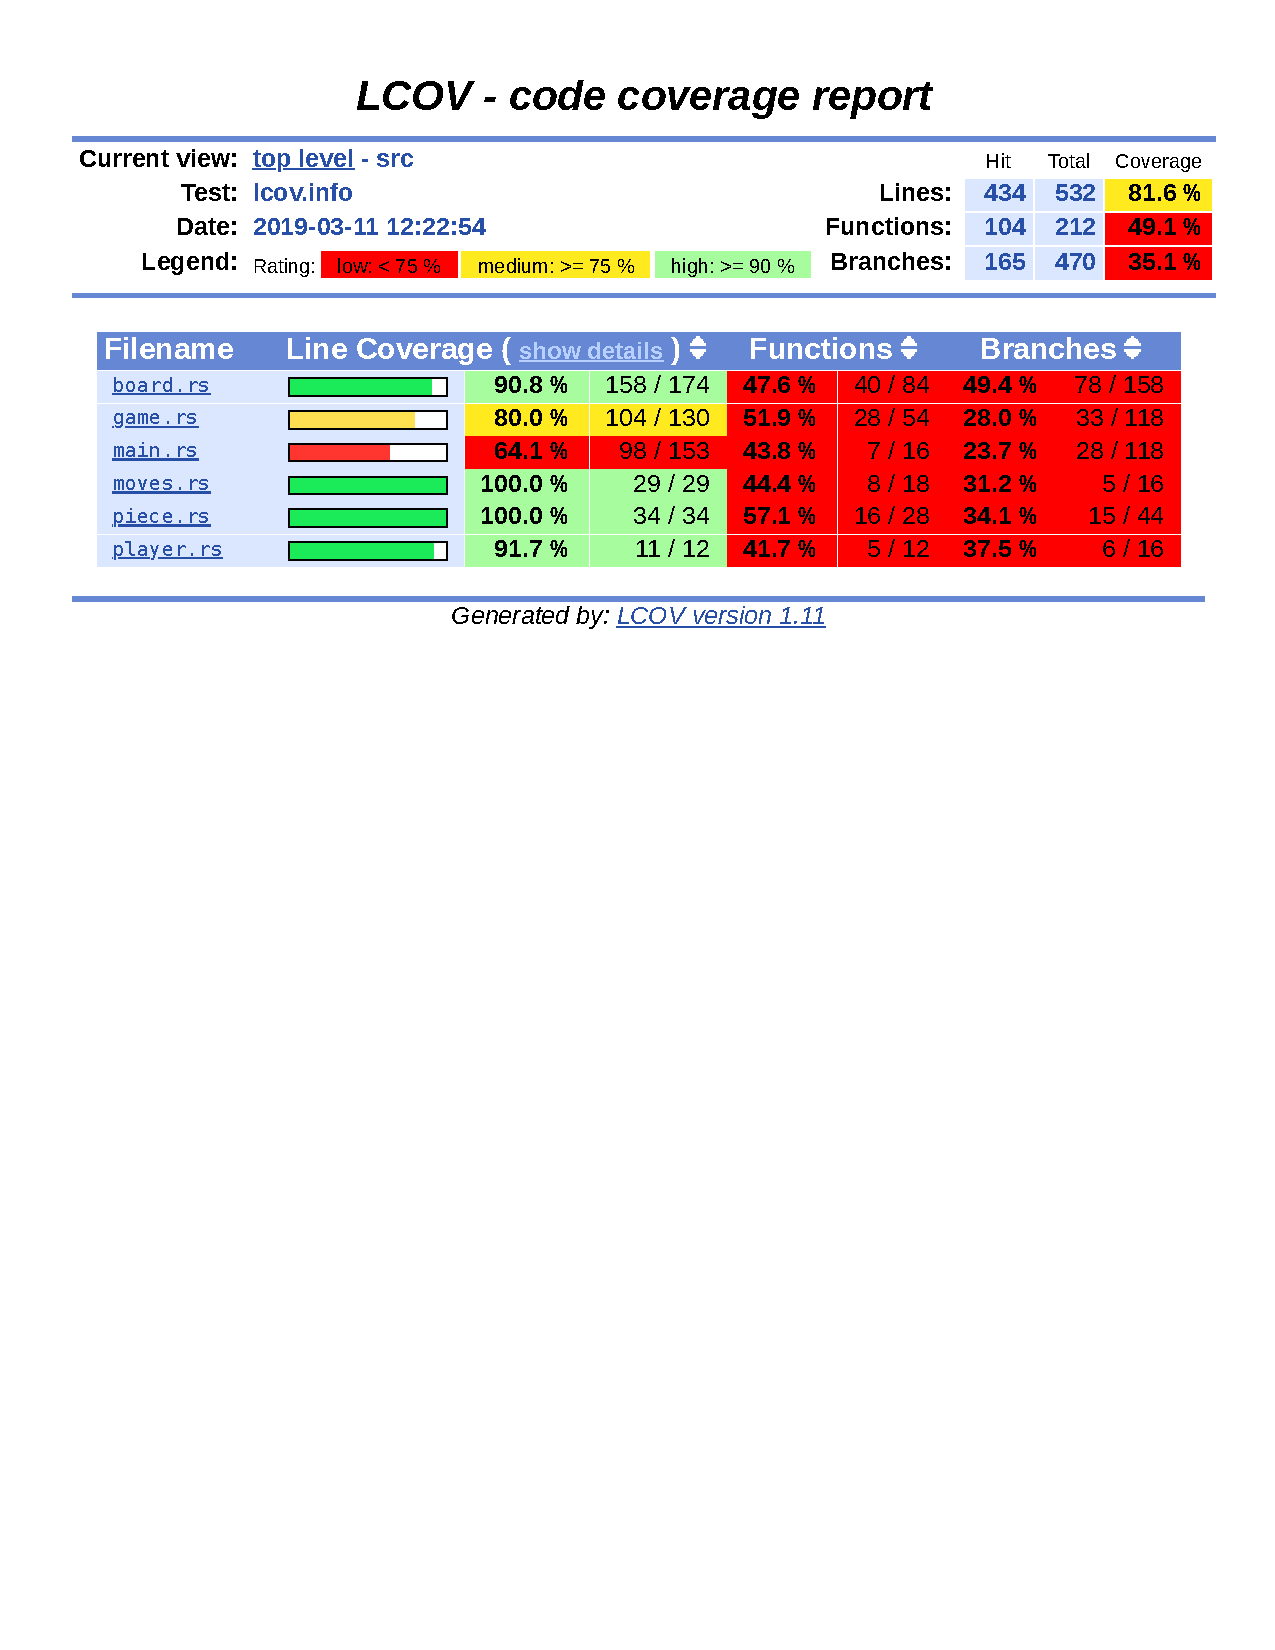
\includepdf[offset=0em -5em,pages=1,pagecommand=\section{Code Coverage}]{lcov_report_0_1_0.pdf}
\includepdf[offset=0em -5em,pages=2-,pagecommand={}]{lcov_report_0_1_0.pdf}

\section{Static Analysis}
The programming language Rust was chosen for development purposes in part due
to its in-built static analysis. With compiler implementations of concepts such
as borrow checking, lifetimes, and ownership, Rust attempts to guarantee memory
safety. By virtue of building without explicitly unsafe sections,
\textsc{Rusted Checkers} passes these static checks.

Extra linting analysis may be run with \texttt{make lint}. Any warnings
existing warnings from this command have been reviewed and allowed by the
developers.

\section{Release Notes}
This document outlines release notes for \texttt{v0.1.0} of \textsc{Rusted Checkers}.
\subsection{Working}
\begin{itemize}
  \item A game is created and a board is displayed within a terminal or TTY console.
  \item Piece capturing is implemented and displays a pieces as being captured.
  \item Possible moves are generated when an owned piece is clicked.
\end{itemize}
\subsection{Not Implemented}
\begin{itemize}
  \item Networking, in full
  \item Piece promotion
\end{itemize}
\subsection{Known Issues}
\begin{itemize}
  \item The main thread may panic on certain clicks that are unbounded by the
    board window.
\end{itemize}

\section{Test Cases}
This document has been created in order to outline the methodologies that were employed in order to
 test the functionality and overall performance of the game of Checkers. These tests evaluate the current 
state of the program in accordance with the requirements stated in the requirements document. Checkers 
is an application that enables two users to play a traditional game of checkers over a local network. 
\subsection{Test Case 1: Initializing the Game}
\subsubsection{Description}
This test case outlines the steps necessary to launch and host a game of Checkers as well as the criteria 
specified for a succesful launch. 
\subsubsection{Pre-conditions necessary for the test case}
The two workstations must be connected over a local network. 
\subsubsection{Scenario}

\begin{center}
\begin{tabular}{ | p{1cm} |p{2cm}|p{2cm} |p{4cm}|p{4cm} |p{1.5cm}|  }\hline

  TestID & Requirement &Description & Execution Steps & Expected Results & Actual Results \\ \hline
	A1 &4.1&Launch Game& Application should be launched by clicking the rust file& A GUI with the splash screen will be displayed to the user. Prompt to press any key to continue to the main screen.&Success\\ \hline
  A2 &4.2&Local Game &Click on the local game button& Navigate to the Local Game Screen&Success\\ \hline
  A3 &4.3&Local Game - Host Game&Click on the Host Game button on Local Game Screen&Server application starts and local IP is displayed.&Fail\\ \hline
  A4 &4.3&Local Game - Join Game&Click on the Join Game button on Local Game Screen&List of hosts on local IP displayed. Text field for input of host IP address is displayed.&Fail\\ \hline
  A5 &4.3&Join Game - Success&Click on a displayed host on Local Game Screen&Request to join game is sent to server on host. Server initiates game between host device and other client. Board UI displayed.&Fail\\ \hline
  A6 &4.3&Join Game - Success&Enter IP address of host server and click "Join" on Local Game Screen&Request to join game is sent to server on host. Server initiates game between host device and other client. Board UI displayed.&Fail\\ \hline
  A7 &4.3&Join Game - Fail&Enter INVALID IP address of host server and click "Join" on Local Game Screen&Request to join game is sent to server on host. Server is not found and error is displayed to user.&Fail\\ \hline
  A8 & -- &Lost Connection - Failure&One client is closed or a connection is dropped.&The remaining client should recieve information about a disconnect and be prompted to exit.&Success\\ \hline
  
\end{tabular}
\end{center}

\subsection{Test Case 2: Playing the Game}
\subsubsection{Description}
The test cases below outline the checks necessary to ensure legal moves are made and that
players are informed as to the status of the board (e.g capture of a piece, change of turn).
\subsubsection{Pre-conditions necessary for the test case}
The two workstations must be connected over a local network. A session should be active between these two 
workstations where a gameboard with pieces is displayed graphically to the two users in real time. 
\subsubsection{Scenario}
\begin{center}
\begin{tabular}{ | p{1cm} |p{2cm}|p{2cm} |p{4cm}|p{4cm} |p{1.5cm}|  }\hline

  TestID & Requirement &Description & Execution Steps & Expected Results & Actual Results \\ \hline
  B1&5.1&Making a Move - Unpromoted Piece Success&Active player moves piece to available position in forward direction&Move data sent to server. Server validates move and sends updated board state to both players. GUI of players updates with board state.&Success\\ \hline
  B2&5.1&Making a Move - Promoted Piece Success&Active player moves piece to available position in either direction&Move data sent to server. Server validates move and sends updated board state to both players. GUI of players updates with board state.&Success\\ \hline
  B3&5.1&Making a Move - Failure&Active player moves piece to INVALID position&Move rejected on client-side and user is informed of invalid move&Success\\ \hline
  B4&5.2&Capturing a Piece - Unpromoted Piece Success&Active player makes required capture move by 'hopping' over enemy piece in forward direction to available square.&Move data sent to server. Server validates move and sends updated board state to both players. GUI of players updates with board state, removing captured pieces.&Success\\ \hline
  B5&5.2&Capturing a Piece - Promoted Piece Success&Active player makes required capture move by 'hopping' over enemy piece in either direction to available square.&Move data sent to server. Server validates move and sends updated board state to both players. GUI of players updates with board state, removing captured pieces.&Success\\ \hline
  B6&5.2&Capturing a Piece - Failure&Active player makes invalid capture or fails to capture&Client informes user of invalid move, failing locally&Success\\ \hline 
  B7&5.3&Promoting a Piece - Success&Active player makes valid unpromoted piece move to last row of board&Move data sent to and validated by server, new board state including the newly promoted piece sent to board players. GUI updated with promoted piece.&Success \\ \hline 

\end{tabular}
\end{center}

\subsection{Test Case 3: Ending the Game}
\subsubsection{Description}
The following test cases outline conditions in which a game between two players may end by a win, resignation, or loss of connection to client/server.
\subsubsection{Pre-conditions necessary for the test case}
The two workstations must be connected over a local network. A session should be active between these two 
workstations where a gameboard with pieces is displayed graphically to the two users in real time. The game 
may be drawing to a close at this point. 
\subsubsection{Scenario}

\begin{center}
\begin{tabular}{ | p{1cm} |p{2cm}|p{2cm} |p{4cm}|p{4cm} |p{1.5cm}|  }\hline

  TestID & Requirement &Description & Execution Steps & Expected Results & Actual Results \\ \hline
  C1&5.4&Game Complete by Win - Success&Active player captures last piece of opponent (one piece left on board)&Move sent to and validates by server. Server informs both players of completed game and ends the game. GUI updates with winner status and users are prompted to exit or play again.&Success \\ \hline
  C2&5.9&Game Complete by Resignation - Success&Active player clicks "Resign" button and confirms prompt.&Move data containing resignation is sent to and validated by server.Server informs both players of completed game and ends the game. GUI updates with winner status and users are prompted to exit or play again.&Success \\ \hline
  C3 & -- &Lost Connection - Failure&One client is closed or a connection is dropped.&The remaining client should recieve information about a disconnect and be prompted to exit.&Success\\ \hline

\end{tabular}
\end{center}


\end{document}
